
This section introduces several techniques used in SLAM and 3D Reconstruction for estimating pose. As mentioned, both of these research areas employ techniques to compute camera pose. Once camera pose is known, in the case of RGB-D methods, depth data may be integrated to generate dense 3D reconstructions. In the case of monocular or stereo approaches, dense depth information may be computed implicitly to varying degrees of accuracy. Once computed it may be integrated in a similar manner to RGB-D based methods. \\

There are many examples of camera pose being computed by robots \cite{Olson06Fast,Frese05Multilevel,Dellaert06Square,Thrun02Robotic,Nuchter056d,Grisetti07Efficient,Kaess08Isam}, in these cases, pose may be estimated by taking input from sensors (measuring wheel spins or thrust) \cite{Callieri04Roboscan}. It can also be computed via more complex methods based primarily on visual data \cite{Davison03Real,Klein07Parallel,Strasdat10Real,Jin00Real,Nister05Preemptive}. 
\\

If only monocular video data is available, the true scale of the map cannot be determined so true measurement based reconstructions are not possible \cite{Endres12Evaluation,Konolige08Outdoor, Paz08Large}. Furthermore many monocular algorithms only produce sparse reconstructions \cite{Davison03Real,Klein07Parallel}. \\

The first monocular slam system was presented by Davison in 2003 \cite{Davison03Real}. Davison's method uses a hand-held camera in real time to produce globally consistent sparse maps. It makes use of probabilistic filtering in its estimates of both camera pose (translation and rotation) as well as triangulation of sparse features. It was successful but is limited to in-door office environments because it requires large state vectors which grow with scene size. Another known limitation is that the use of sparse feature maps leads to poor accuracy. \\

Later, systems which split tracking and mapping (global optimization) came along such as the Parallel Tracking and Mapping Algorithm (PTAM) \cite{Klein07Parallel}. PTAM also performs camera tracking in real-time in small work spaces. It is essentially a bundle adjustment (a least squares solution to camera and feature optimization see section \ref{sec:ba}) based pose estimation procedure. The tracking system runs in parallel at frame-rate speeds, performing robust n-point pose estimation with feature matching. In comparison to filter based methods, much more features can be packed into the map \cite{Strasdat10Real}. Approaches such as these typically accumulate drift (such as work by Beardsley et al \cite{Beardsley97Sequential}) or perform off-line loop-closure optimization. \\

\subsection{The Fundamental Matrix and its Properties}

\label{FundamentalMatrixSection}

The Fundamental matrix method is especially useful in systems where monocular cameras are used for 3D reconstruction. From 2D point correspondences, the fundamental matrix may be computed. This leads to both the direct estimation of camera pose as well as stereo calibration parameters (which are required to compute dense depth information from monocular views). Here the Fundamental and Essential matrices, their estimation, properties and use in pose estimation are described.

To describe this technique, linear algebra is used. Note, all of the transforms required to represent imaging systems can be represented using $4 \times 4$ matrices and homogeneous $4 \times 1$ vectors. These important transforms include: 3D rotation, scaling, shearing/skewing, mirroring, translation and perspective transforms. Rather than describing camera capture using projecting rays, linear algebra provides further capabilities and clearly defines the estimation process of the fundamental matrix. 

In figure \ref{fig:INTRO_FMA1} there are two camera systems. Next an explanation as to how point $Q$ is projected from 3D onto the 2D point $Q_{1}$ is discussed. First, $C_{1}$ is defined as the origin (later this allows rotation and perspective transforms to more easily be performed). In order to do this, $C_{1}$ can be subtracted from itself (to become the origin) and so it is also subtracted from $Q$ as well. To this end, a $4 \times 4$ translation matrix, $T$ is used. Next, rotation is performed in order to align the camera's axes with the x, y and z axes. The camera's axes can be defined using three vectors. One pointing directly ahead where the camera is facing (piercing the center of the projection frame), another points directly to the right perpendicularly (orthogonal to the first), the final points above the camera, aligned orthogonally with the previous two vectors. \\

These three axes can be placed into the columns of a $4 \times 4$ homogeneous matrix. This forms a matrix which rotates an aligned camera's axis to face the direction where $C_1$ currently points to. In other words, it performs the exact opposite of what is needed. Since this matrix is orthogonal (known because the column vectors are all perpendicular) the inverse transform is simply the transpose of this matrix. This rotation matrix is defined as $R$. Next, there may be a lateral alignment, this is a translation which further aligns the points to the center of the frame. This is performed using another $4 \times 4$ matrix, $L$. Finally, another $4 \times 4$ matrix, P is used to project the point $Q$ to the 2D point, $Q_1$. The entire projection can be performed by multiplying these matrices together, $Projection = P * L * R * T$. Here, $P * L$ are known as the intrinsic parameters whilst $R * T$ are called the extrinsic parameters. Due to the imperfect nature of the camera lens, the intrinsic camera matrix often has distortion, this becomes important later when we define the difference between the fundamental matrix and another matrix introduced, the essential matrix.

\begin{figure*}[!htb]
	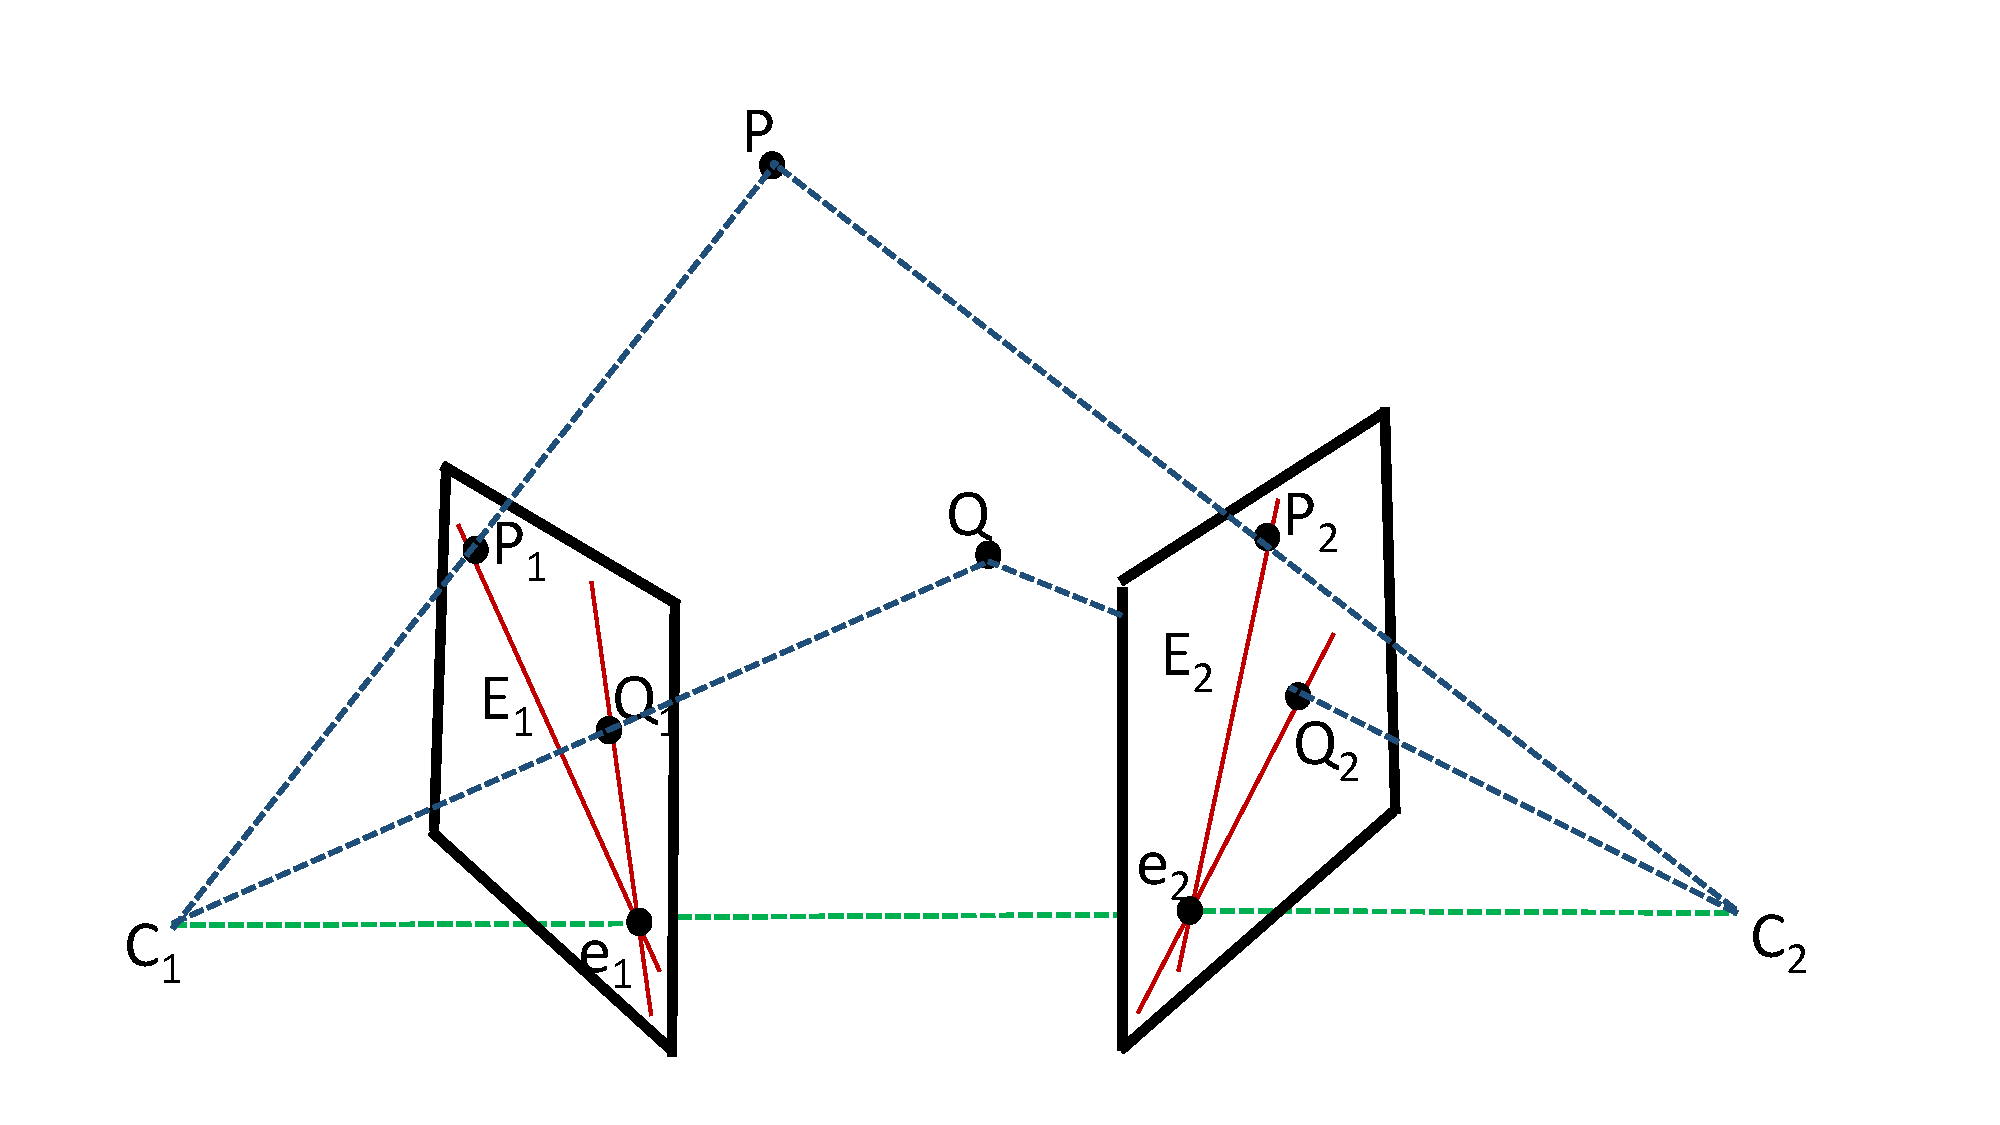
\includegraphics[width=5.0in]{images/introfm1}
	\caption{A pair of cameras viewing two points. This figure is a reconstruction of the figure on page 492 in Computer and machine vision: theory, algorithms, practicalities \cite{Davies12Computer}.}
	\label{fig:INTRO_FMA1}
\end{figure*}  

Using the steps described and looking at figure \ref{fig:INTRO_FMA1}, it has been identified how 3D point $P$ is mapped to both of the frames with cameras $C_1$ and $C_2$. Projecting point $P$ onto the two frames gives points $P_1$ and $P_2$ respectively. $V_1$ is defined as a vector relating $P_1$ and $P_2$. It is formed by normalising the vector from $C_1$ to $P$, and $V_2$ (normalizing $(P - C_1)$. The relation between between these vectors is the essential matrix \cite{Davies12Computer}, $E$. The specific relation is $V_2^{T} * E * V_1 = 0$. The depth of $P$ is unknown and cannot be estimated directly unless an investigation is performed on the particular camera system in use. The precise perspective transform and associated distortion must be known. Fortunately, both the depth and the perspective are cancelled in this matrix formulation, and so we can specify the relation using only the 2D points, $P_1^T * E * P_2 = 0$. \\

This formula is based on the assumption that no distortion is present in the camera system. In this case, both of the cameras may have distortion. We represent this distortion here using matrices $G_1$ and $G_2$. If both shots are taken with the same camera, it is assumed that $G_1$ is equal to $G_2$. We therefore relate the theoretically precise $P_1$ and $P_2$ with their real world equivalents (which have distortion) $D_1$ and $D_2$ by $P_1 = Q_1^{-1} * D_1$ and $P_2 = Q_2^{-1} * D_2$. Inserting this into the essential matrix formulation we have, $(Q_1^{-1} * D_1)^T * E * Q_2^{-1} * D_2 = D_{1}^{T} * {Q_1^{-1}}^{T} * E * Q_2^{-1} * D_2 = 0$. The presence of this distortion is the difference between the essential and fundamental matrices with the fundamental matrix being $F = {Q_1^{-1}}^{T} * E * Q_2^{-1}$. If no distortion is present, the fundamental matrix is equivalent to the essential matrix. \\

Using the Essential or Fundamental matrices, we may compute both camera pose, and stereo calibration. The camera pose is computed by using singular value decomposition (SVD) on the essential matrix. This breaks it down =into 3 matrices ($W$, $U$ and $V$). Then, both the translation part (equation \ref{eqn:FundaTrans}) and rotational part (equation \ref{eqn:FundaRote}) of the camera pose may be computed.


\begin{equation} \label{eqn:FundaTrans}
Translation Matrix = W\left[
\begin{array}{ccc}
0 & 1 & 0 \\
-1 & 0 & 0 \\
0 & 0 & 0 \\
\end{array}
\right]W^{T}
\end{equation}

\begin{equation} \label{eqn:FundaRote}
Rotation Matrix = W\left[
\begin{array}{ccc}
0 & -1 & 0 \\
1 & 0 & 0 \\
0 & 0 & 0 \\
\end{array}
\right]V^{T}
\end{equation}

Looking at figure \ref{fig:INTRO_FMA1} again, line $E_1$ represents an epipolar line, this line lies on the plane in which both cameras and point $P$ lie on. Line $E_1$ is the epipolar line belonging to the left frame and $E_2$ is the epipolar line belonging to the right frame. Point $e_1$ is the epipole of the left frame and point $e_2$ is the epipole of the right frame. Epipoles are the projection of one camera's location onto the frame of another camera. The projection of $C_2$ onto the left frame by camera $C_1$ is the epipole $e_1$. If the fundamental matrix is multiplied by a particular point it produces a vector in $R^3$ which represents the epipolar line as $[a b c]^T$ in which $a,b$ and $c$ represent the line equation $ax^2 + bx + c$. The epipolar line corresponding to $Q$ and $Q_1$ passes through a common point with the other epipolar line $E_1$. All epipolar lines intersect at the epipole. \\

The fundamental matrix may be computed using point matches between images. As mentioned the fundamental matrix can be used to perform image rectification and estimate camera pose. As shown, the fundamental matrix, epipolar lines and epipoles can be estimated from point correspondences. If the epipoles are known, then the direction in which the other camera resides is also known. \\

The basic pipeline for the fundamental matrix method begins with feature matching. Using matches, the fundamental matrix is estimated usually using an outlier filtering strategy such as Random Sample Consensus RANSAC. Then extrinsic camera information is estimated and images are rectified and so that disparity information can be computed. This may be used to compute dense depth data required for 3D reconstruction. One downside to this method is that the scale of the translation computed is not to scale. \\


Monocular Feature based SLAM systems use feature matches to estimate camera pose and location changes across frames \cite{Davison02Simultaneous}. Variations of this method use different features including: corners and lines \cite{Jeong06Visual}, image patches \cite{Silveira08Efficient} and exemplar feature matching \cite{Chekhlov07Robust}. SIFT features are used most often in SLAM \cite{Jensfelt06Framework,Pollefeys08Detailed,Beall11Bundle,Eudes10Fast}, in addition FAST features have been explored \cite{Kundu10Realtime,Leelasawassuk133d,Konolige10View,Konolige08Frameslam}. Beall et al \cite{Beall11Bundle} made use of both SIFT and SURF features in their underwater SLAM system. Real-time monocular SLAM systems based on this approach have also been proposed \cite{Chekhlov07Robust,Pollefeys08Detailed}. RANSAC is often used in monocular SLAM \cite{Eudes10Fast,Kundu10Realtime,Konolige10View,Konolige08Frameslam,Pradeep13Monofusion} to remove outliers. Without RANSAC, incorrect camera parameter estimates would prevent any accurate pose estimation in all but synthetic data. Bundle adjustment is also used as an additional step to refine camera parameter estimation \cite{Eudes10Fast} (section \ref{sec:ba}).  \\


\subsection{Feature Matching and RANSAC}
\label{FMANDFM}

Feature matching along with RANSAC  may be used to compute the Fundamental/Essential matrices which leads to camera pose estimates. However, the computation of the correct Fundamental matrix is typically difficult. Furthermore, the intrinsic camera parameters must be known prior in order to use such a technique, else noise destroys the ability to accurately estimate camera pose. \\

Another, more common way to use feature matching with RANSAC \cite{Fischler81Random,Chen99Ransac} is to compute the camera pose directly using RGB-D data. As covered in section \ref{DepthDataGenSection}, dense depth information may be computed using monocular, stereo or sensor based camera set-ups. This method begins by computing feature matches between two given frames. These matches along with the 3D location of each corresponding match (projected using the dense depth data) are injected into the popular Random Sample Consensus Algorithm commonly known as RANSAC. RANSAC is an iterative algorithm which works by repeatedly selecting a subset of input data, computing a model on the subset and testing that model on the global superset. During this repeated process, the subset with the best classification (lowest error or greatest strength model) is chosen for the final model. RANSAC is useful because it is capable of filtering out outliers. \\

In the case of camera pose estimation, the subset is used to compute the camera pose (using singular value decomposition) and the camera pose which minimizes the global error is chosen as the best camera pose. Here we describe how to compute the camera pose given a set of 3D points matched from one frame to another. Given two identical length arrays of 3D points, $P$ and $Q$ where, for each index $i$, $P_i$ matches best with $Q_i$. Next, we compute covariance matrix $X$ based on $P$, $Q$ and their mean values. The calculation for $X$ is shown in figure \ref{eqn:CovarMatForFMRansac}.


\begin{equation} \label{eqn:CovarMatForFMRansac}
X = \sum_{i=1}^{N} (P_i - P_{mean}) \times (Q_i - Q_{mean})^T
\end{equation}

Given the covariance matrix $X$ we compute its singular value decomposition matrices $W$, $U$ and $V$ (was usv). Then the rotation part of the pose may be computed as $R = V^T \times U^T$. The camera movement can be computed by $T = -R \times P_{mean} + Q_{mean}$. If scale must be computed, it can be computed as $S = (Q_i - Q_{mean}) / (R \times(P_i - P_{mean}))$ for any $i$. \\

Computing 3D reconstructions using feature matching is often preferred as close competitor ICP (Iterative Closest Point) is often unnecessary and expensive \cite{Endres12Evaluation}. However, the computation of pose without ICP with feature matching only is non-trivial because the system may suffer from the following issues:


\begin{itemize}
\item Synchronization problems between the RGB camera and Infrared camera shutters
\item depth jump interpolation - the interpolation of computed depth at object boundaries
\item feature matches often occur at depth jumps
\end{itemize}



\subsubsection{RGB-D SLAM}

Endres et al \cite{Endres12Evaluation} presented a dense 3D reconstruction technique using RGB-D data from the Kinect sensor based on feature matching and RANSAC. They also evaluated their technique under different illumination and camera movement speed conditions. It is able to operate at near real time speeds in small in-door environments. This method begins by feature matching RGB images across frames. Using the projected 3D points available for each pixel in the depth map, RANSAC \cite{Fischler81Random,Huttenlocher91Fast} is used to compute the camera pose across frames. These poses are optimized globally using the $g^2$o graph optimizer, the Octomap representation \cite{Wurm10Octomap} is used to voxelize the 3d points before storing them in a volumetric occupancy map. Since this system is based on feature matching, Endres et al evaluate 3 different feature matching techniques: SIFT \cite{Lowe04Distinctive} , SURF \cite{Bay06Surf,Bay08Speeded} and ORB \cite{Rublee11Orb}. ORB feature matching is tested because it is faster than SIFT and SURF with slightly less accuracy, the authors also evaluate a GPU implementation of SIFT \cite{Wu07Siftgpu}. Endres et al evaluate their algorithm using their own benchmark \cite{Sturm11Towards}. Results show it can handle up to 50 degrees of rotation per second, and speeds of up to 43 centimetres per second.  \\


This system is divided into a front-end and a back-end. The front-end performs feature detection, matching and sensor pose estimation via the RANSAC method whereas the back-end performs non-linear pose optimization using the $g^2o$ optimization procedure   and integrates these results into an occupancy grid based on the Octomap. A diagram of the combined front-end and back-end systems is given in figure \ref{Endres12EvaluationPipeline}. 


\begin{figure}[!h]
\centering
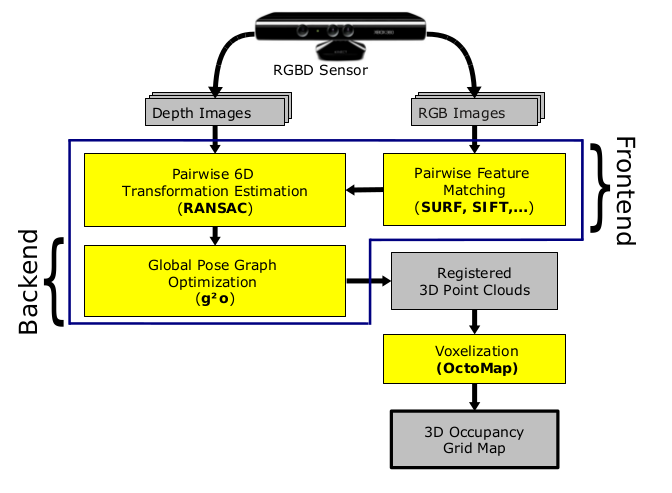
\includegraphics[width=12cm]{images/ch1/Endres12EvaluationPipeline}
\caption{RGB-D SLAM Pipeline used by Endres et al \cite{Endres12Evaluation}}
\label{Endres12EvaluationPipeline}
\end{figure}


The front-end uses OpenCV \cite{Bradski08Learning} for feature matching. During the feature detection process, the Hessian threshold is used to keep the total number of features constant. This is required because pose may not be able to be computed if there aren't enough features, but on the other hand, too many features typically lead to many false positives in the feature matching schema. As mentioned, these matched features (and thus matched 3d points) are used with RANSAC to compute pose \cite{Umeyama91Least}. During the RANSAC process, corresponding points with distances below 3cm are considered inliers. The inliers are then used exclusively to compute a finer pose. This method of pose estimation is fast but computational complexity depends on the number of features computed. For each frame, the pose relationship with 20 previous frames (including the most recent 3) is computed in parallel on the GPU. Then the final computed pose is given to the back-end. If accurate pose cannot be compute, constant motion is assumed. \\

\subsubsection{Fast Odometry from Vision: FOVIS}

Another technique which is based on feature matching is the FOVIS (Fast Odometry from Vision) technique \cite{Huang17Visual}. In FOVIS works in 6 stages. In the first two stages, the RGB-D image data is collected and put through a low-pass filter, Gaussian scale space is computed and then FAST features \cite{Rosten06Machine,Rosten05Fusing} are computed. In the next stage, initial camera rotation estimation is computed by minimizing the sum of squared errors between down sampled versions of consecutive image frames. In the 4th stage, feature matching is performed, using the SAD (sum of absolute differences) metric and sub-pixel resolution. In the 5th stage, outliers are removed using a feature match graph and a greedy algorithm to find maximal cliques \cite{Hirschmuller02Fast,Howard08Real}. \\

In the final stage, the full camera pose is estimated by first computing it using Horns method \cite{Horn87Closed} This technique minimizes an error function in computing the camera rotation and translation. The FOVIS method then optimizes this by minimizing the re-projection error using a non-linear least squares method. \\

Whelan et al \cite{Whelan12Kintinuous} extended Kinectfusion allowing it to map larger areas. They compared ICP with FOVIS and found that FOVIS contributed less drift but lack-luster models compared with ICP. Whelan et al also proposed a technique for incrementally creating a triangle mesh as the reconstruction was built. This method uses multi-threadeding, and uses pose graph optimization (see section \ref{Sec:G20}).



\subsection{ICP}

\label{ICPSection}

Iterative Closest Point (ICP) \cite{Besl92Method,Rusinkiewicz01Efficient,Segal09Generalized} is a non-linear optimization method used to register 3D data. It works by iteratively minimizing registration error given two sets of point clouds and is a popular method for estimating 6-dof (6 degrees of freedom) camera alignment in 3D reconstruction. The algorithm works by computing the closest point using some metric (usually euclidean distance) for each of the points in the first point cloud. Then computing a transform which minimizes either the euclidean distance error or some other error metric (\cite{Steinbrucker11Real,Tykkala11Direct,Kerl13Robust,Chen92Object,Stuckler12Robust}. \\

The points are then transformed by the computed transform and this process is repeated which is supposed to continually decrease registration error. The 6-dof are commonly computed using the method described in section \ref{FMANDFM}. Various distance metrics have been researched including the point-plane metric \cite{Chen92Object}. This metric improves convergence rates and is used for surface reconstructions which contain additional information about the normal of each points. This algorithm is highly successful in generating accurate 3D reconstructions but it does have a few issues. \\

The first issue is that whilst computing the best transform based on "feature matches" based on closest points is relatively simple, computing these closest points for each input point is expensive. This can be improved using the projective data association algorithm \cite{Blais95Registering} usually used by exploiting a projected version of the 3D data. The efficiency issue can also be improved using a coarse to fine scheme. \\

Another issue that ICP is limited to small rotation, translation and scale. If larger transforms are present (especially scale in the case of general registration) ICP will usually get stuck in a local minima and fail to register \cite{Mitra04Registration}. The final issue is that of slippage \cite{Whelan13Robust}. ICP tends to fail in environments with little texture. Here we present some important algorithms which use ICP in 3D reconstruction.

\subsubsection{Feature Matching, RANSAC and ICP Refinement}

Some systems make use of feature matching with RANSAC (see section \ref{FMANDFM}) for pose estimation and ICP for further alignment \cite{Engelhard11Real, Henry10Rgb}. These methods are very similar and make use of the advantages of both the feature matching methods and ICP method. \\

Henry et al \cite{Henry10Rgb} presented work on a 3D mapping method which combines Feature Matching and RANSAC (similar to \cite{Endres12Evaluation}) with ICP. This method makes us of an RGB-D camera, and used the camera input for sparse feature matching. Features are used with RANSAC and the technique described in section \ref{FMANDFM}. ICP is used for refinement of the initial prediction. If Loop-closure is detected, a constraint is added to the 3D pose graph \cite{Kummerle11G} and is used to close the loop. A Surfel \cite{Pfister00Surfels} volumetric fusion method is used to represent and store the 3D reconstruction. This technique may be used for robot localization and path planning \cite{Hornung10Humanoid}. Endres et al \cite{Endres12Evaluation} compared this method with theirs using a standard benchmark \cite{Sturm12Benchmark}.  \\

\subsubsection{Non-Rigid Alignment}

In addition to rigid alignment ICP is used by Pauly et al \cite{Pauly05Example,Brown07Global} to align depth maps using non-rigid transforms. In the method by Brown and Rusinkiewicz \cite{Brown07Global}, ICP is used to first align the point clouds using a rigid alignment, then global feature positions are found using a relaxation method. Then 3D point sets are warped to final positions using thin plate splines. Brown and Rusinkiewicz state that this outperforms rigid based alignments.


\subsubsection{Kinect Fusion}

Newcombe et al \cite{Newcombe11Kinectfusion,Izadi11Kinectfusion} proposed an accurate, real-time dense 3d reconstruction algorithm which works well on complex indoor environments. This algorithm computes relationships between depth map frames generated using the Microsoft Kinect \cite{Zhang12Microsoft} sensor. By aligning depth maps this method is capable of tracking both camera pose and location as well as generating dense 3d reconstructions. Only depth data is used in alignment computations thus, consequently because the Kinect is a structured light based depth sensor Kinect Fusion works under any lighting condition, including complete darkness. Since they use the Kinect and GPU (both considered commodity hardware these days) the technique may be considered inexpensive. \\

The method works by computing camera pose, transforming depth data by a computed pose (frame-by-frame) and fusing this data into a global surface volume. It uses a coarse to fine grain iterative closest point (ICP) algorithm to compute camera pose. During the ICP phase, the target points come from the entire globally matched previous frames. Therefore this method is considered global rather than frame-to-frame based. Such a method has direct advantages over frame-by-frame feature matching, since all data is used to compute pose. The downside, is that this method fails to find global solutions due to the nature of ICP. This may occur when some frames must be skipped due to motion blur, or the camera passing over surfaces which do not reflect infra-red light. \\

\begin{figure}[!h]
\centering
%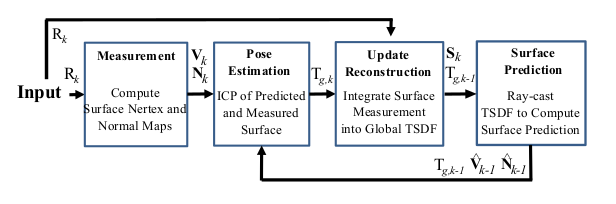
\includegraphics[width=12cm]{images/ch1/Newcombe11KinectFusion1}
\caption{Kinect Fusion Algorithm Pipeline \cite{Newcombe11Kinectfusion}}
\label{KFusionPipeliciteHne}
\end{figure}

Kinect Fusion has four main steps as illustrated in figure \ref{KFusionPipeline}. The first step named measurement, performs pre-processing on the depth data as well as generation of additional information for use by Kinect Fusion. Each depth map frame is first passed through a bilateral filter. From this, a dense vertex map (map of 3D points projected using a known projection matrix associated with the Kinect) is generated, as well as a normal map. For both the vertex and normal maps, a 3 level image pyramid is constructed. This makes the coarse to fine grain ICP technique possible. \\

Next, dense coarse to fine grain ICP is used to compute pose between the fused frames and the current frame. The authors exploit the fact that the transformation between frames is small because camera motion is slow when computing against every frame. With coarse-to-fine grain ICP they use projective data association \cite{Blais95Registering} and the point-plane metric for pose optimization \cite{Rusinkiewicz02Real}. The ICP based pose estimation computes pose given both a predicted and measured depth map. \\

After estimating camera pose relating to the globally fused model, each frame must be integrated into that model. The Kinect Fusion algorithm uses a truncated signed distance function (TSDF) representation. This is a signed distance function volume where the distances for each voxel are capped by some value. The TSDF uses a volume resolution of $512\times 512\times 512$. They use the TSDF, rather than relying on a linear but accurate discrete SDF transform \cite{Rasch09Remarks} because of the computational complexity of calculating the discrete SDF of large scale volumes. \\

As mentioned, Kinect fusion uses pose prediction and fuses each depth map into the TSDF representation. In this way, they align and fuse each depth map to the global 3d reconstruction. In this way, a global loop closure method is not required. This may have a negative side effect by which some frames which have larger resolutions may be heavily quantized in order to fuse with the SDF, especially very thin surfaces/objects. These features may also be advantageous for ICP in estimating pose. 


\subsubsection{FOVIS and ICP Integration}

Whelan et al improved \cite{Whelan13Robust} upon their previous method \cite{Whelan12Kintinous} by integrating FOVIS and ICP together on the GPU, and adding an advanced colour fusion model to the technique. The main improvement lies in switching between FOVIS and ICP whenever the error using FOVIS is too high, ICP is used. They also integrate using a global model rather than a local one. 


\subsection{Direct Optimization Methods}

\subsubsection{Optimization over a Signed Distance Function}

In 2013, Bylow et al \cite{Bylow13Real} presented a novel method which reconstructs static indoor environments in real time using RGB-D data captured using the Asus Xtion Pro Live sensor. Their system is able to generate accurate 3D RGB coloured models of the environment in real-time by optimizing for 6 degrees of freedom in terms of accurate projection of new depth map frames into an existing global signed distance function model of the scene. Their method uses several Gauss Newton optimization with a signed distance function representation, these techniques are represented and processed using a laptop with an NVIDIA GPU. Unlike Kinect Fusion \cite{Newcombe11Kinectfusion}, this method optimizes directly in the signed distance representation, in which camera pose is computed by finding a rotation and translation (6-DoF) which minimizes the error of projecting depth images into the SDF. Compared with the ICP based method used by Kinect Fusion, this technique is shown to be more robust and accurate. It compares favourably to bundle adjustment but is much faster for small to mid sized scenes. Results are generated using the TUM RGB-D benchmark and SDF volume sizes $256^3$ and $512^3$ are used in evaluations. The authors note the algorithm may be able to handle large scale scenes if used in conjunction with other techniques \cite{Kaess11Isam2,Kummerle11G}. \\

This technique is efficient because the error to minimize can be checked using several look-ups since the SDF itself contains the distances from each voxel to the global model's actual surface. Because of this, the algorithm is classified as working within global space rather than frame-by-frame. Using the SDF to lookup depth map projection error, the camera pose is iteratively estimated and then the depth map is integrated into the SDF and colour information is stored in another volume. The pose estimation procedure begins by storing the first frame as a volumetric signed distance function. Then for each new depth frame, camera pose is computed, and based on this pose the frame is projected into the scene. Using a lie algebra based 6-DoF model \cite{Ma12Invitation} envisioned as a vector in $R^6$ representing camera pose, the error for a given pose may be computed as the squared error of the depth map transformed by the pose and projected into the signed distance function. Due to noise or missing data within the depth frame, this error may never be reduced completely, instead the best pose is iteratively computed using this model and the Gauss Newton non-linear optimization algorithm. \\

The SDF representation uses two volumes as in \cite{Curless96Volumetric}, one volume stores the average distances, the other stores the cumulative weights for each voxel. Bylow et al use these weights to handle occlusion and sensor uncertainty. When integrating a point into the SDF, tri-linear interpolation is used between eight neighbours to handle point coordinated made up of floating point numbers. During integration, each voxel is projected onto the image plane rather than ray case from the center of projection as in \cite{Newcombe11Kinectfusion}. This ensures that each voxel is visited once when updating the SDF, whereas in the ray casting approach, this may not necessarily be the case. \\

In computing the SDF for a given depth map, the exhaustive marching cubes algorithm is too slow, even the fast marching algorithm \cite{Baerentzen01Implementation} is not suited for real time discrete SDF generation. Instead, the SDF is approximated with either the point to point distance or point to plane distance functions. For final visualization, marching cubes is used \cite{Lorensen87Marching} on the final SDF. Colour is computed from the colour volume using a technique found used by Whelan et al \cite{Whelan13Robust}. Since the method by Bylow et al is based on optimizing the projection error using the SDF and only uses locations in its pose estimation procedure, it is independent to illumination. Given this, it will also fail in cases where only co-planar surfaces are visible, they mention that using colour information during tracking \cite{Kerl13Robust} may mitigate these concerns.

\subsubsection{ICP + SDF Optimization}

Rusinkiewicz et al \cite{Rusinkiewicz02Real} developed a 3D reconstruction technique based on frame-by-frame ICP and integration using an occupancy grid. Users scan small objects by rotating them by hand. Output models are optimized using an SDF \cite{Curless96Volumetric}.


\subsubsection{Warp Function Optimization} 

Kerl et al \cite{Kerl13Dense} proposed a dense RGB-D SLAM system which uses a probabilistic camera parameter estimation procedure. Rather than strictly using feature matching, RANSAC and a linear pose estimator, it formulates the projection error as an image warping function (between two frames) and optimizes it using Taylor's expansion.

\subsubsection{Event Feature Optimization}

Weikersdorfer et al \cite{Weikersdorfer14Event} presented a novel sensor system named D-eDVS along with an event based SLAM algorithm. The D-eDVS sensor combines depth and event driven contrast detection. The event emitting sensor can be thought of as emitting points which may be used like features. After aligning pixels generated from the event transmitting device with depth information from the Asus Xtion pro RGB-D camera, it computes pose by optimizing the re-projection error using least squares optimization.


\subsection{3D Feature Matching}

3D feature matching works much in the same way as the 2D feature matching and RANSAC approach (section \ref{FMANDFM}) but uses 3D features rather than 2D only, so it can work independently to perspective changes which 2D feature matching methods are only robust to. Many techniques have been proposed \cite{Scovanner073Dimensional,Flitton10Object,Li05Multiscale}. Technically, registering against rigid transformations may be achieved with as little as 3 feature matches. These 3 matches can be found by 3D feature matching or geometric hashing \cite{Wolfson97Geometric}.



\subsubsection{4-Point Congruent Sets}

Aiger et al \cite{Aiger084} developed a method for 3D registration (and pose estimation) named 4-Point Congruent Sets (4-PCS). This method is fast and robust to wide baselines in the registration of 3D data. It is resilient to noise and outliers and there is no pre-filtering or de-noising required prior to registration. It improves the typical feature matching approach by significantly reducing the number of points required to compare as features for use in a RANSAC approach to pose estimation. \\

This method works by extracting all co-planar 4 point sets from a 3D point cloud which are congruent (under a rigid transformation) to a given set of co-planar 4-points. The complexity of this method is $O(N^{2k})$ where N is the number of points and k is the number of 4-point sets. When there is not too much noise, this method may use feature matching only which brings the complexity down to $O(N+k)$. Aiger et al also presented an extension to register against affine transforms. This method was tested with varying levels of noise, outliers and and overlap. \\

This method works based on the principal of large numbers, which means solving the largest common point-set (LCP) problem. This problem states, given to point-sets $P$ and $Q$, LCP under δ-congruency solves for a subset $P_i$ of $P$ having the largest cardinality such that the distance between $T(P_i)$ and $Q$  is less than δ given an appropriate distance measure (T is a rigid body transformation). \\

The basic concept is to optimize the selection of the 3 points used as a base for alignment from one point-set to another. By choosing 3 matches, then measuring the distance between $T(P_i)$ and $Q_i$. This test is of complexity  O($m^3$ x $n^3$) but this can be reduced to  O($mn^3 log(n)$) \cite{Irani96Combinatorial} and even O($n^3 log(n)$). Despite these improvements, these complexities are still too large for practically sized point-sets. This novel 3D alignment scheme is capable of aligning surfaces with limited overlap and may be refined using ICP \cite{Rusinkiewicz01Efficient}. \\


\subsubsection{Base Shape Matching}

Gelfand et al \cite{Gelfand04Shape} presented a method which segments input models into base shapes, simple geometric parts which may be modelled and matched. Using these base shapes, slippable components are found by computing local slippage signatures for a set of points in the input and iteratively clustering regions with matching slippable motions. This method is stable but appears to be limited to mechanical human made parts and shapes.

\subsubsection{Multi-scale Features}

Extensions to both SIFT and SURF have been extended to 3D \cite{Scovanner073Dimensional,Flitton10Object}. These methods follow the same overall technique as the 2D counterparts however some procedures and practices are altered to better suit 3D data input. First, a 3D-volume scale pyramid is produced for matching at different scales. Then features are detected using the corresponding feature detection method (by SIFT or SURF) and then a feature vector for each feature is produced. Features can be matched between volumes and a rigid or non-rigid alignment may be computed. \\

Li and Guskov \cite{Li05Multiscale} developed a 3D feature matching technique based on 3D SIFT for SURFEL (3D point and normal) data. It computes a scale space pyramid using a per point scheme in which the next scale up for each point and corresponding normal is computed as the point which minimizes an error function. Salient features are then computed using the scale space. Features are those points which maximize (or minimize) a measurement based on dot product of the normal and the difference between points at adjacent scales. \\

Li and Guskov use their technique to find approximate transformations, then ICP is used for further alignment \cite{Besl92Method,Chen92Object}. This technique is slow for data-sets with large amounts of input data, yet it does not work well with sparse data-sets. \\

	
Mori et al \cite{Mori05Efficient} proposed a matching method based on two levels: a high level matching method which is used to compute a short-list for candidates and a low level method which is more computationally complex. This technique is simply used for matching and uses larger areas rather than local features like SIFT 3D. \\

Other 3D feature matching techniques which have been developed are based on images \cite{Wolfson97Geometric,Johnson97Spin}. In these techniques features are typically described using some sort of 2D image function rather than a single dimensional vector. Typically a normal is computed for a feature point and some projection is used to compute an image which is used as a descriptor. Then these features may be matched between 3D volumes using normalized cross-correlation or another image comparison method.  \\

Some feature matching techniques are based on hashing or voting \cite{Germain97Fingerprint,Gal06Salient,Mitra04Registration,Ballard91Generalizing}. These techniques are out of the scope of this research but are none the less interesting areas which are still underdeveloped.


\subsection{Principal Components Analysis}

Principal Components Analysis (PCA) is an algorithm which divides a set of observed vector data into their principal component vectors and a centroid. The vectors along with the principal axes may be used to align 3D data. An issue with PCA is that in the case of partial overlap, the accuracy may break down \cite{Aiger084}. The Principal Components Analysis algorithm and it's use in the proposed technique is discussed in section \ref{FullRecovery3DSection}. \\

Pottmann et al \cite{Pottmann07Principal} showed that PCA performed on local neighbourhoods is able to compute principal directions and curvatures at a given scale which can be used for feature matching. \\





